\documentclass[12pt,a4paper]{article}
\usepackage[utf8]{inputenc}
\usepackage{amsmath}
\usepackage{amsfonts}
\usepackage{amssymb}
\usepackage{verbatim}
\usepackage[margin = 2cm]{geometry}
\usepackage{graphicx}
\usepackage{listings}
\usepackage{xcolor}
 
\definecolor{codegreen}{rgb}{0,0.6,0}
\definecolor{codegray}{rgb}{0.5,0.5,0.5}
\definecolor{codepurple}{rgb}{0.58,0,0.82}
\definecolor{backcolour}{rgb}{0.95,0.95,0.92}
 
\lstdefinestyle{mystyle}{
    backgroundcolor=\color{backcolour},   
    commentstyle=\color{codegreen},
    keywordstyle=\color{magenta},
    numberstyle=\tiny\color{codegray},
    stringstyle=\color{codepurple},
    basicstyle=\ttfamily\footnotesize,
    breakatwhitespace=false,         
    breaklines=true,                 
    captionpos=b,                    
    keepspaces=true,                 
    numbers=left,                    
    numbersep=5pt,                  
    showspaces=false,                
    showstringspaces=false,
    showtabs=false,                  
    tabsize=2
}
 
\lstset{style=mystyle}




\author{Steven Maharaj\\695281}
\title{Code task 1}

\begin{document}

\maketitle

\section*{a}
The \texttt{LCG\_alogorithm} in the \texttt{LCG} module implements the LCG alogrithim. 
\begin{lstlisting}[language=Python, caption=LCG.LCG\_alogrithm]
def LCG_alogorithm(a,b,m,seed = 2,iterations=20):
    """"
    Implements the LCG alogrithm 
    Outputs: an array of random numbers of size iterations x 1
    """
    x = np.zeros(iterations)
    x[0] = seed

    for i in range(1,iterations):
        x[i] = (a*x[i-1] + b)%m
    return x
\end{lstlisting}
\texttt{a\_test.py} tests the algorithm.



\begin{lstlisting}[language=Python, caption=\texttt{a\_test.py}]
from LCG import LCG_alogorithm

print(LCG_alogorithm(a =2,b=0,m=7))


\end{lstlisting}

\texttt{a\_test.py} yields the following output

\begin{verbatim}
[2. 4. 1. 2. 4. 1. 2. 4. 1. 2. 4. 1. 2. 4. 1. 2. 4. 1. 2. 4.]
\end{verbatim}

\section*{b}

The \texttt{check\_valid } in the \texttt{LCG} module check if a sequence of random numbers is valid.

\begin{lstlisting}[language=Python, caption=\texttt{LCG.check\_valid}]
def check_valid(x,m):
    """Checks if a sequence x is vaild
    
    Inputs: x - sequence
            m 
            
    Output : True if valid
             False if not valid"""
    n_non_repeating = np.argwhere(x[0] == x).flatten()[1] 
    if n_non_repeating==m-1:
        vaild = True
    else:
        vaild = False

    return vaild
\end{lstlisting}

\texttt{b\_test.py} checks the valid value of $a$ when $b=0, m=7$.

\begin{lstlisting}[language=Python, caption=\texttt{b\_test.py}]
from LCG import LCG_alogorithm, check_valid

b,m = 0,7
for a in range(1,m):
    x = LCG_alogorithm(a,b,m,seed = 2,iterations=20)
    if check_valid(x,m):
        print(f"a = {a} is valid")
\end{lstlisting}
We find that

\begin{verbatim}
a = 3 is valid
a = 5 is valid
\end{verbatim}

\section*{c}
For the valid values of $a$, values 1 to 6 is are uniform distributed like a real dice. However, the numbers repeat after $m-1$ realisations . This makes the random numbers predictable thus the model specified in part b is inadequate. 

\section*{d}

\texttt{d\_test.py} checks the number valid when $b=0, m=997$.

\begin{lstlisting}[language=Python, caption=\texttt{d\_test.py}]
from LCG import LCG_alogorithm, check_valid

b,m = 0,997
count = 0
for a in range(1,m):
    x = LCG_alogorithm(a,b,m,seed = 2,iterations=2000)
    if check_valid(x,m):
        count += 1

print(f"There are {count} vaild")
\end{lstlisting}
\begin{verbatim}
There are 328 vaild
\end{verbatim}

\section*{e}
\texttt{d\_test.py} simulates dice throws for $a = 825, b=0, m=997$.

\begin{lstlisting}[language=Python, caption=\texttt{e\_test.py}]
from LCG import LCG_alogorithm

a,b,m = 825,0,997
x = LCG_alogorithm(a,b,m,seed = 2,iterations=50)
dice_throws = (x%6)+1
print(dice_throws)
\end{lstlisting}

\texttt{e\_test.py} yield the follow output.
\begin{verbatim}
[3. 6. 4. 1. 6. 2. 6. 4. 2. 2. 1. 3. 3. 1. 3. 5. 5. 3. 1. 3. 6. 6. 2. 3.
 6. 3. 2. 2. 4. 5. 2. 3. 4. 3. 1. 3. 3. 6. 1. 2. 4. 5. 2. 6. 3. 5. 4. 1.
 1. 5.]
\end{verbatim}


\section{f}
\texttt{f\_test.py} performs 10000 iterations.
\begin{lstlisting}[language=Python, caption=\texttt{f\_test.py}]
from LCG import LCG_alogorithm,prob_of_two_sixs
import matplotlib.pyplot as plt
import seaborn as sns
sns.set_style("darkgrid")

a,b,m = 825,0,997
x = LCG_alogorithm(a,b,m,seed = 2,iterations=10000)
dice_throws = (x%6)+1

probabilty_of_two_sixs = prob_of_two_sixs(x)

print("For 10000 dice rolls")
print(f'The empirical probabilty of rolling two sixs is {probabilty_of_two_sixs}')

# Plots
hist = sns.countplot(x=dice_throws)
plt.xlabel("Dice values")
plt.ylabel("Freqency")
plt.title("Dice throws")
plt.savefig("fig/dice_freqency",dpi=250)
plt.show(hist)
\end{lstlisting}

Figure \ref{fig:dice_throws} shows that the empirical probabilities are uniform. For example the probability of rolling a 1 and the probability of rolling a 5 are the same.

For a real dice the probability of roll two sixes in a row is $1/36$ . However, from our simulation

\begin{verbatim}
The empirical probabilty of rolling two sixs is 0.0
\end{verbatim}
Therefore this suggests the algorithm can not sufficiently model a random dice roll for this choice of parameters.

\begin{figure}
\centering
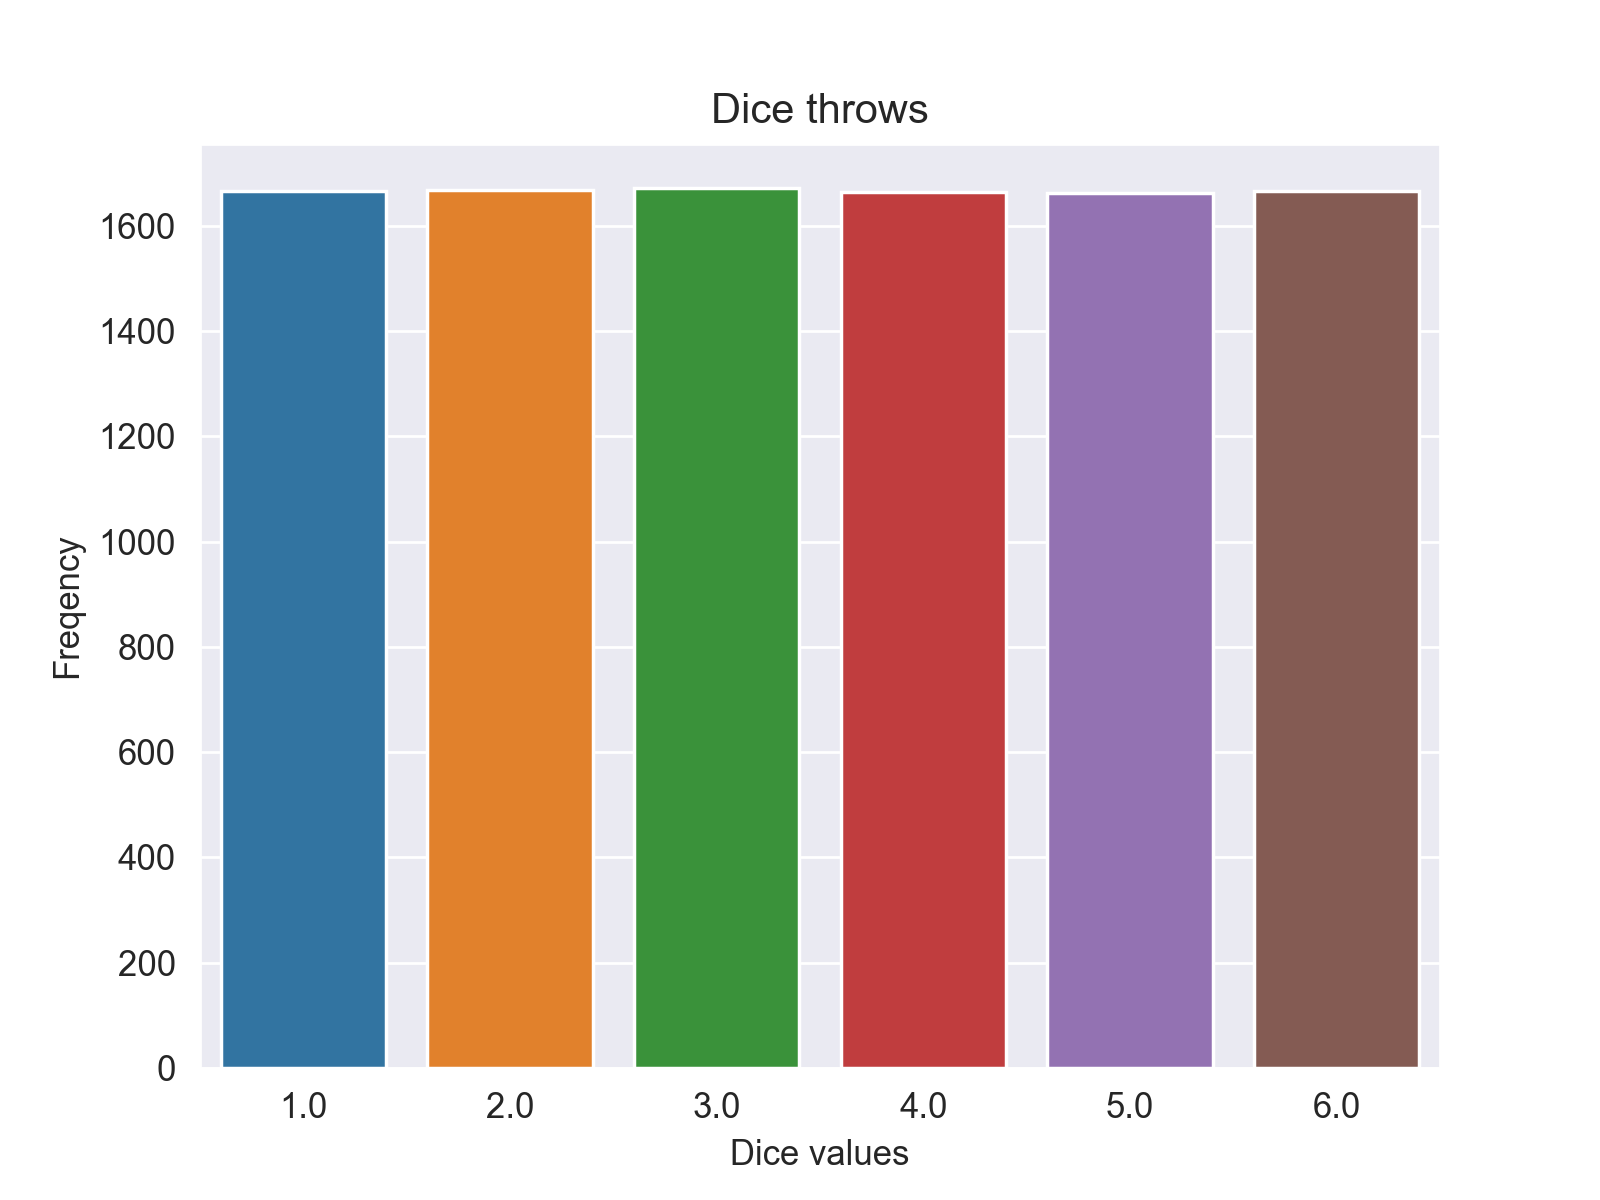
\includegraphics[scale=0.7]{../fig/dice_freqency.png}
\caption{Frequency of each dice throw. Performed for 10000 iteration. a,b,m = 825,0,997.}
\label{fig:dice_throws}
\end{figure}


\section*{g}
If let $a= 858$ and us the same parameter from question f, the probabilities are not uniform. Figure \ref{fig:dice_throws_bad} shows a clear non-uniform distribution. Thus, the values chosen for the parameters $a,b,m$ are very important as they greatly impact how how ‘random’ the generated values from the LCG algorithm.

\begin{figure}
\centering
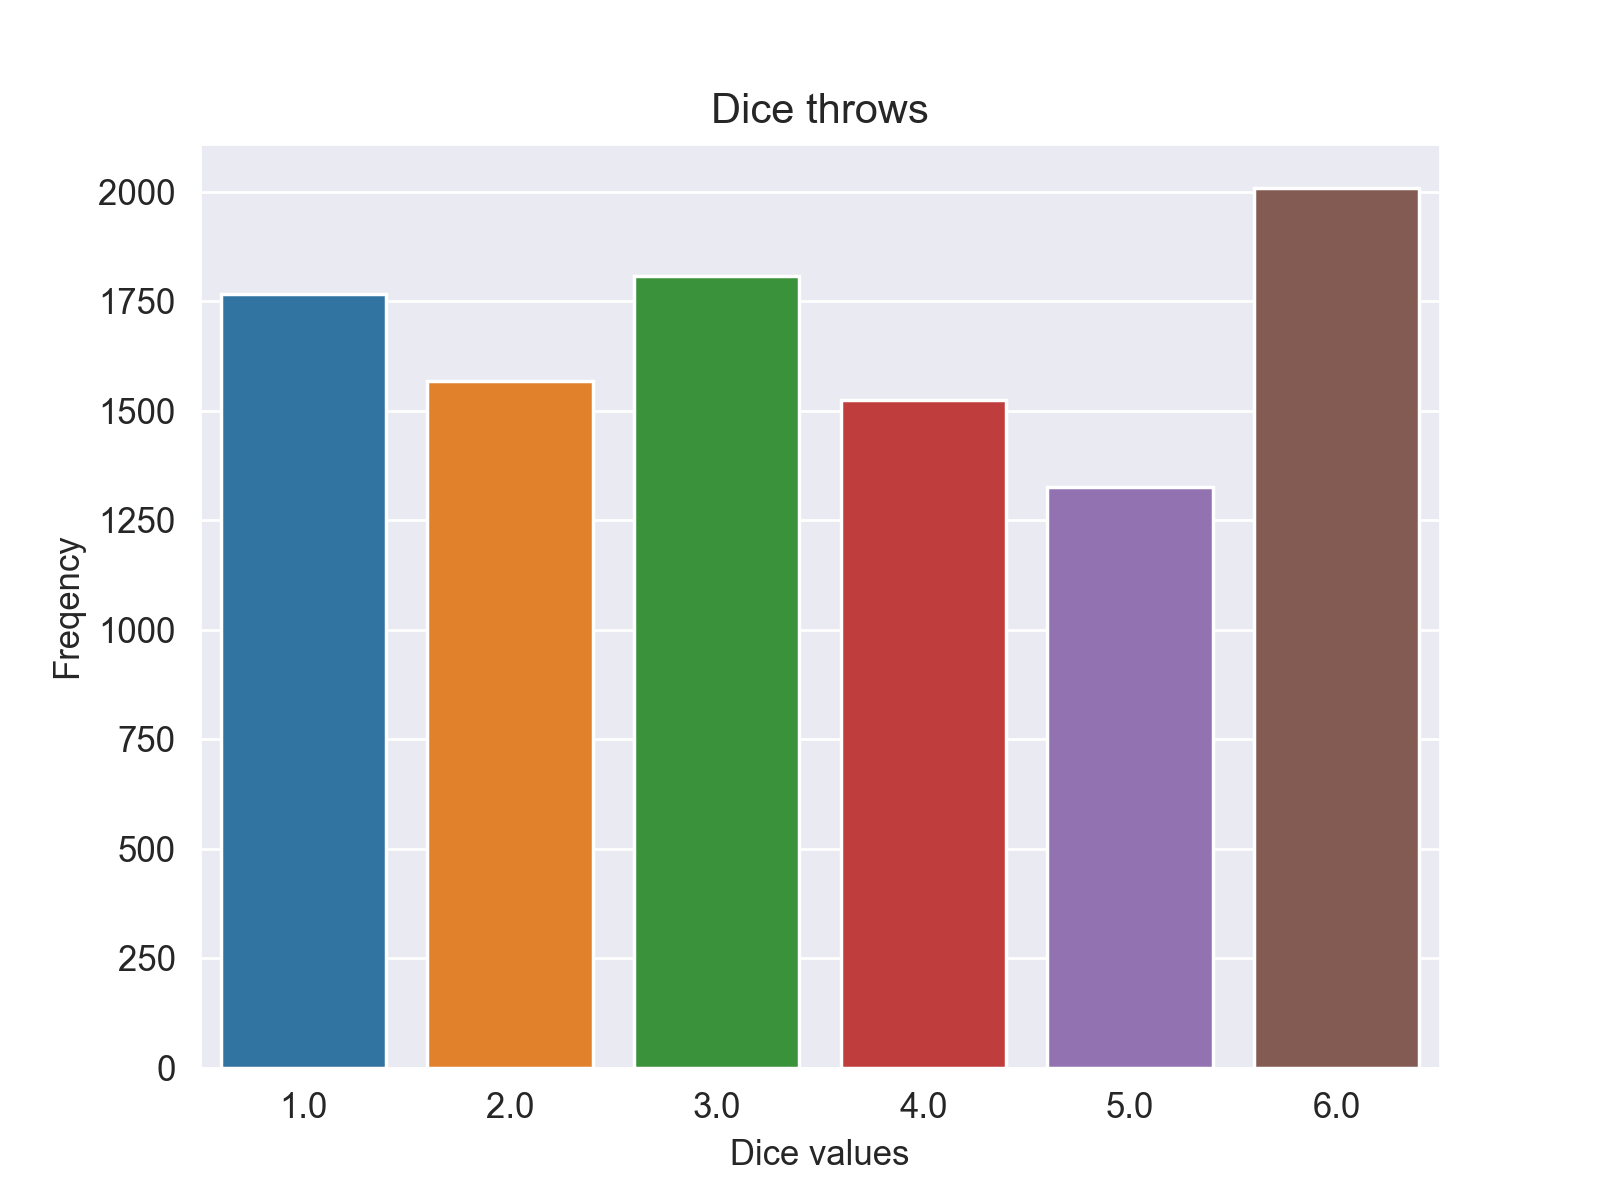
\includegraphics[scale=0.7]{../fig/dice_freqency_bad.png}
\caption{Frequency of each dice throw. Performed for 10000 iteration. a,b,m = 858,0,997.}
\label{fig:dice_throws_bad}
\end{figure}
\end{document}